\setbeamercolor{background canvas}{bg=fitblue}
\begin{frame}
\frametitle{Transform feedback}
\begin{center}
\Huge {\color{white}Transform feedback}
\end{center}
\end{frame}
\setbeamercolor{background canvas}{bg=white}

\begin{frame}
\frametitle{Transform feedback}
	\begin{itemize}
	\item Zápis primitiv do bufferu
	\item Hlavně v Geometry Shaderu
	\item Streams (kreslení i zápis o bufferu)
	\end{itemize}
	\begin{figure}[h]
	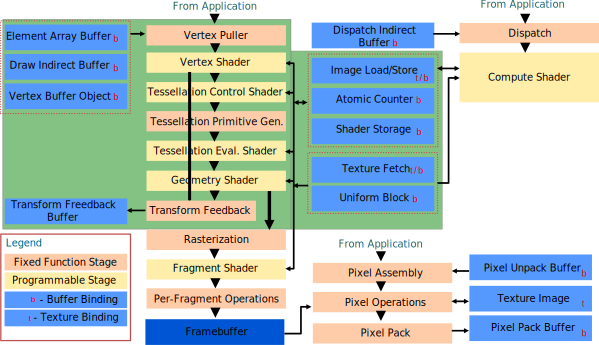
\includegraphics[width=10cm,keepaspectratio]{pics/transformFeedback/tf_pipeline}
	\end{figure}
\end{frame}

\begin{frame}
\frametitle{Transform feedback}
	\begin{figure}[h]
	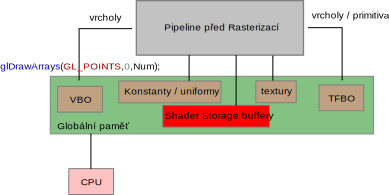
\includegraphics[width=10cm,keepaspectratio]{pics/transformFeedback/tf_mem}
	\end{figure}
\end{frame}

\begin{frame}[fragile]
\frametitle{Transform feedback - příklad}
	{\scriptsize
	\begin{minted}[frame=lines]{c++}
const char*Vayrings[]={"Out1", "Out2"};
glTransformFeedbackVaryings(Program,2,Varyings,GL_SEPARATE_ATTRIBS);
glLinkProgram(Program);

//...

glBindBufferBase(GL_TRANSFORM_FEEDBACK_BUFFER,0,Buffer1);
glBindBufferBase(GL_TRANSFORM_FEEDBACK_BUFFER,1,Buffer2);

glEnable(GL_RASTERIZER_DISCARD);//nebudeme rasterizovat
//...
glBeginTransformFeedback(GL_TRIANGLES);
glDrawArrays(...);
glEndTransformFeedback();
	\end{minted}
	}
\end{frame}

\begin{frame}[fragile]
\frametitle{Transform Feedback - Inicializace}
	Slinkovat program s nastavenými výstupními proměnnými v shaderu.
	c++:
	{\scriptsize
	\begin{minted}[frame=lines]{cpp}
//seznam promennych v shaderu, ktere se budou pomoci TF zapisovat do bufferu
const char*ResetVaryings[]={"vPosition","vVelocity","vMass"};
//nastavime seznam a nastavime prokladany zapis
glTransformFeedbackVaryings(ResetProgram,3,ResetVaryings,GL_INTERLEAVED_ATTRIBS);
//znovu slinkujeme program
glLinkProgram(ResetProgram);
	\end{minted}
	}
	glsl:
	{\scriptsize
	\begin{minted}[frame=lines]{glsl}
#version 330

layout(location=0)out vec2  vPosition;//pozice castice
layout(location=1)out vec2  vVelocity;//rychlost castice
layout(location=2)out float vMass;//hmotnost castice
//...
void main(){
  vPosition = vec2(0);//pozice do prostred
  vVelocity = vec2(cos(VelAngle),sin(VelAngle))*VelSize;//rychlost jako vektor
  vMass     = Noise(MassSeed+uint(gl_VertexID),MinMass,MaxMass);//hmotnost
}
	\end{minted}
	}
\end{frame}

